\chapter{Evaluation}

\section{Real problem application}

In this section, we will try to suggest a couple of problems where the ScalaAdaptive library could be used to improve the overall performance. The problems will be described and an example usage of the library will be provided, along with evaluation of its effects.

\subsection{JSON parsing}

JSON\footnote{JavaScript Object Notation} is a data-exchange format that can hold serialized object trees and collections based on the notation for object (technically key-value dictionaries) literals in JavaScript. The format has recently become extremely popular due to its simplicity, data efficiency and readability, and as of today, is basically a standard for communication HTTP REST APIs. Most of the systems with distributed architecture that communicate over such an API (typically client-server applications) need to serialize and deserialize JSON upon sending a request or receiving a response, which might occur quite often.

%TODO: A lot of abbreviations here...

The problem concerning JSON and other similar formats (XML, ProtocolBuffers, etc.) is that there is a variety of libraries available to perform the serialization and deserialization, and we have to decide for one when designing our application. The API tends to be very similar, and for many systems, the performance might be the issue. There are performance tests available that compare the performance of the libraries, but the performance might be different for various sizes, structures, etc. In addition, in the \textit{Capturing Performance Assumptions using Stochastic Performance Logic} it is shown that the performance might vary in different versions.
%TODO: Add reference and VERIFY!!!

This library decision problem is a perfect use-case for ScalaAdaptive - we can create a simple wrapper library with the same API as the original libraries that will expose the functions combined from the original serialization and deserialization methods. The user will be abstracted from the ScalaAdaptive, and the libraries can be added or removed at any time very easily.

\subsubsection{Combining GSON and Jackson}

For the test, we will use two JSON libraries - GSON and Jackson, which are probably two of the most common libraries from the Java world. We will measure only the deserialization part (parsing of string containing JSON), which is the more time-complex operation. A library wrapper that exposes three parsing functions was created:
\begin{itemize}
	\item \inlinecode{parseWithGson()}
	\item \inlinecode{parseWithJackson()}
	\item \inlinecode{parse()} - previous two methods combined using ScalaAdaptive
\end{itemize}

The setup for the test is following:
\begin{itemize}
	\item TTestSelectionStrategy with $\alpha = 0.05$
	\item PauseSelectionAfterStreakPolicy with streak length 10 and retry every 200th run
\end{itemize}

The grouping applied is logarithmic to the JSON input string length, i.e. $groupId = log(length)$. We expect different behavior for different groups. We will use three different JSON strings for the test:

\begin{itemize}
	\item Small - 9KB, 10 records array
	\item Medium - 80KB, 100 records array
	\item Large - 8MB, 1000 records array
\end{itemize}

We know that we will deal with fixed sizes of input files, so we can use the t-test selector without any problems, because every size will occupy one of the groups. If we knew that the sizes within a group might vary, we should use some other strategy.

During the test, we ran each one of the three parsing functions 10000 times on the small JSON, 5000 times on the medium JSON and 200 times on the large JSON. We measured the total run time of all the functions, and the results can be seen in the table \ref{tab:json_parsing_results}. The measurements are in miliseconds and include complete runs of the parsing functions, including the overhead of ScalaAdaptive.

\begin{table}[h!]
\captionsetup{justification=centering,margin=0.5cm}
\bgroup
\def\arraystretch{1.5}%
\begin{center}
	\begin{tabular}{ | l | r | r | r | }
		\hline
		& \textbf{GSON} & \textbf{Jackson} & \textbf{Combined} \\ \hline
		10000 * Small JSON & 1830.36 & 4883.24 & 2566.54 \\ \hline	
		Small JSON average & 0.18 & 0.49 & 0.26 \\ \hline	
		5000* Medium JSON & 4865.89 & 3142.05 & 3059.18 \\ \hline	
		Medium JSON average & 0.97 & 0.63 & 0.61 \\ \hline	
		200 * Large JSON & 15790.47 & 7298.75 & 7740.31 \\ \hline	
		Large JSON average & 78.95 & 36.49 & 38.70 \\ \hline
		Total time & 22486.71 & 15324.05 & 13366.03 \\
		\hline
	\end{tabular}
\end{center}
\egroup
\caption{Results of the JSON parsing tests (times in ms).}
\label{tab:json_parsing_results}
\end{table}

As we can see, the average time in all cases is roughly the same or a little worse than the time of the better alternative. The total time spent on parsing shows us that without using ScalaAdaptive, we would get worse performance no matter which function we used.

We can compare the results with table \ref{tab:json_parsing_results_no_policy} showing the same test, only without the PauseSelectionAfterStreakPolicy. We see that by actually performing the selection every time, the overhead grows, which can be best seen on the small and medium inputs, where the results are significantly worse.

\begin{table}[h!]
		\captionsetup{justification=centering,margin=0.5cm}
	\bgroup
	\def\arraystretch{1.5}%
	\begin{center}
		\begin{tabular}{ | l | r | r | r | }
			\hline
			& \textbf{GSON} & \textbf{Jackson} & \textbf{Combined} \\ \hline
10000 * Small JSON  & 2180.20       & 5615.20          & 5667.64           \\ \hline
Small JSON average  & 0.22          & 0.56             & 0.57              \\ \hline
5000 * Medium JSON  & 4696.52       & 2944.04          & 3889.25           \\ \hline
Medium JSON average & 0.94          & 0.59             & 0.78              \\ \hline
200 * Large JSON    & 15829.39      & 7433.50          & 7772.41           \\ \hline
Large JSON average  & 79.15         & 37.17            & 38.86             \\ \hline
Total time          & 22706.11      & 15992.73         & 17329.30          \\ \hline
		\end{tabular}
	\end{center}
	\egroup
	\caption{Results of the JSON parsing tests without the PauseSelectionAfterStreakPolicy (times in ms).}
	\label{tab:json_parsing_results_no_policy}
\end{table}

\subsection{Load balancing}

A different sort of problems that ScalaAdaptive might help with is to adapt the system to the environment changes. We can demonstrate this on a simple example - the system that relies on a remote web service that runs in multiple instances on different web servers. The service itself is stateless, so we can perform the request on either of them. 

Main goal of the replication is to distribute the work between more nodes, so that the response time remains low. A technique called load balancing should take care of distributing the requests evenly between the nodes often just using a simple round-robin technique. This, however, has to be done on the side of the service, through a common gateway. We will use the ScalaAdaptive to implement a simple load balancing on the side of the client (so that balance between services hosted at different locations could be done) by evaluating the response times and selecting the target node using our selection strategies. We will take advantage of the possibility to limit the maximal duration of historical data - we want to decide based only on the most recent measurements, because we suppose that they will change rapidly.

There are two goals of this load balancing example:

\begin{itemize}
	\item To provide better performance than relying just on one node
	\item To limit the load on the node that is currently under pressure (and thus slow)
\end{itemize}

Suppose we have a simple web service running on multiple nodes and a system that performs synchronously running requests to these nodes. The request has the following function form:

\lstset{style=Scala}
\begin{lstlisting}
def request(url: String)(query: String): Option[String] = ???
\end{lstlisting}

We can take advantage of the possibility to curry the function and create the composed request that works with multiple nodes using the ScalaAdaptive API in the following way:

\lstset{style=Scala}
\begin{lstlisting}
val balancedRequest =
(
  urls.tail.foldLeft(performRequest(urls.head) _) { (f, url) =>
    f.or(performRequest(url)) } 
  selectUsing Selection.NonPredictive 
  limitedTo Duration.ofSeconds(20)
)
\end{lstlisting}

For the actual test, we used two instances of the web server running on different ports of the same machine. We simulated the problems with load on the machines by artificially changing the response times of the servers every 50 seconds according to a set of predefined scenarios. From the client application, we sent one request every 0.5 seconds directly to each one of the servers and one using our balanced method. The results for three different scenarios can be seen in figure \ref{fig:load_balance_scen}. The lines represent response time evolution in time - direct requests are marked with blue and orange, the balanced request is gray. We can observe that most of the time, the gray line copies the lower of the two remaining lines. Sometimes, the gray line repeatedly reaches the higher line, which means that the balanced request is sent to the slower server in order to gather fresh run data.

\begin{figure}[h!]
	\captionsetup{justification=centering,margin=0.5cm}
	\centerline{
		\mbox{
			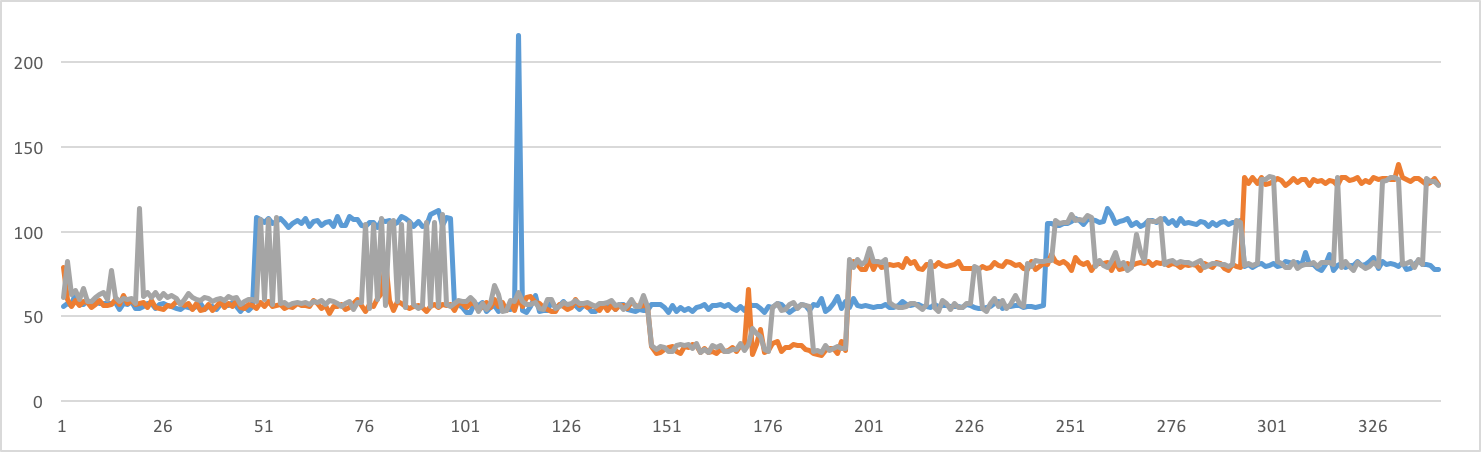
\includegraphics[width=110mm]{./img/load_balance_scen1.png}
		}
	}
	\centerline{
		\mbox{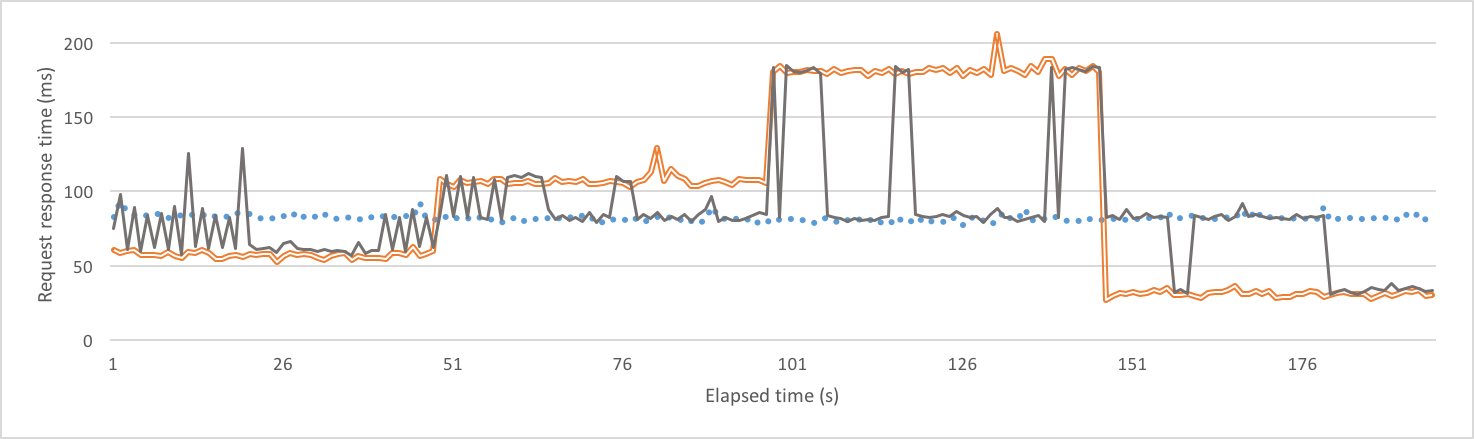
\includegraphics[width=110mm]{./img/load_balance_scen2.png}}
	}
	\centerline{
		\mbox{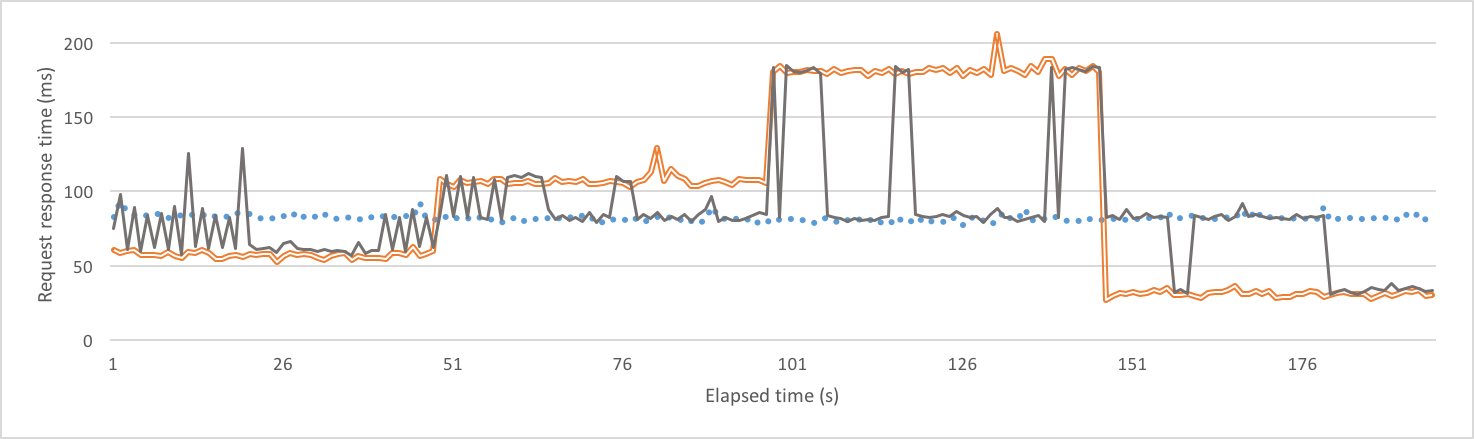
\includegraphics[width=110mm]{./img/load_balance_scen3.png}}
	}
	\caption{Time evolution of response times for request methods in scenarios 1, 2 and 3 (from top to bottom).}
	\label{fig:load_balance_scen}
\end{figure}

The average response times in these scenarios are shown in the table \ref{tab:load_balance_resp_avgs}. The balanced response time is always lower than the worse of the response times. In case where the load alternates between the two servers (scenario 2), the balanced version has the best average response time. If, on the other hand, only one server fluctuates and the other one keeps a relatively low response time (scenario 3), the balanced version is slightly worse than the server that doesn't fluctuate. Nevertheless, the second goal of moving the load between the servers is completed in all three scenarios.

\begin{table}[h!]
	\centering
	\captionsetup{justification=centering,margin=0.5cm}
		\bgroup
	\def\arraystretch{1.5}%
	
	\begin{tabular}{|l|r|r|r|}
		\hline
		& \textbf{Server 1} (blue)& \textbf{Server 2} (orange)& \textbf{Balanced} (gray)\\ \hline
		Scenario 1 & 74.20             & 70.48             & 68.38             \\ \hline
		Scenario 2 & 80.92             & 81.77             & 72.52             \\ \hline
		Scenario 3 & 81.97             & 94.39             & 85.38             \\ \hline
	\end{tabular}
	\egroup
	\caption{Average response times for the request methods in scenarios 1, 2 and 3 in miliseconds.}
\label{tab:load_balance_resp_avgs}
\end{table}

A disadvantage of ScalaAdaptive that complicates the usage in this area is the fact that it doesn't support measuring run times of asynchronous functions, i.e. functions that perform callbacks or complete promises upon finishing.

\section{Spark}

Apache Spark is a framework for distributed computing that is focused on data processing in a similar way to the MapReduce distributed computation paradigm. It works with distributed data sets that can be mapped, filtered, grouped or reduced, but unlike common implementations in Hadoop or other systems, it is focused on in-memory data processing on the nodes. Currently, it is one of the most used systems in distributed big data processing, designed to work with a large variety of distributed storage systems (HDFS, Cassandra, OpenStack Swift).

The Spark framework represents one of the most interesting possibilities to use the ScalaAdaptive framework. The data processing queries are long-running tasks, so any overhead imposed by the selection is negligible. On the other hand, the potentially saved time on a faster implementation increases. In addition, the distributed computation model and the necessity to create an execution plan which depends on the data locations, sizes, etc. leads to large differences in execution times based on:

\begin{itemize}
	\item The query itself
	\item The cluster it is running on (number of machines, cores, network)
	\item The configuration of Apache Spark
\end{itemize}

The goal of this section is to show the basic ideas where the adaptivity might be used in such a framework.

\subsection{Spark APIs}
\label{subsec:spark_apis}

Spark currently supports three different APIs that can be used to construct Spark queries.

\subsubsection{RDD}

RDD (Resilient Distributed Dataset) was the first API introduced and is basically a distributed dataset of JVM objects, which can be queried using higher order functions like \inlinecode{map()}, \inlinecode{filter()}, etc. Spark isn't aware of structure of the internal JVM objects, it is treating the individuals like blackboxes. The query is typed and constructed using lambda expressions that work with these objects. It gets executed when a function that doesn't produce new RDD is called, e.g. \inlinecode{collect()} or \inlinecode{count()}. 

\lstset{style=Scala}
\begin{lstlisting}
rdd.filter(_.id > 5000).count
\end{lstlisting}

Upon execution, the Spark worker engine works with the RDDs as a whole (partitions it, collects the results, etc.), but the operations on its members (filtering, transformation, grouping) are carried out by actually executing the lambda functions. This approach is very simple and allows the user to write queries over custom data types without any limitation. The downside is that the Spark execution engine doesn't know what is going on within the lambdas, can't optimize the execution plan based on the query, and, when moving the parts of RDDs between the nodes, the objects have to be serialized and deserialized again.

\subsubsection{DataFrames and Spark SQL}

DataFrames API was introduced later into the Spark framework with a goal of achieving better performance and scalability. The data within DataFrames are described by a schema, somehow similar to classic SQL schema - Spark knows exactly how are the data records structured. The queries are constructed using Spark SQL, a query language (DSL in Scala) that uses string names of the record attributes (or columns). As we can see in the following example, the actions are described by strings and parsed by Spark upon execution.

\lstset{style=Scala}
\begin{lstlisting}
df.filter("id > 5000").count
\end{lstlisting}

Spark therefore knows how exactly the mapping, filtering, reducing or grouping is going to happen and the Spark can use these information to optimize the execution, data distribution, can use it to make estimations, etc. when building the query plan. In addition, the data described by a schema can be easily persisted or transfered between nodes without the need to perform a JVM serialization. A major disadvantage is the necessity to provide the schema and the fact that the actual query is parsed at runtime and is untyped - errors in attribute names or conditions in general won't be detected upon compilation.

\subsubsection{Datasets}

The newest Spark API, Datasets, was introduced with a goal of combining the best from RDD and DataFrame approaches together. The query programming API is typed and works with JVM objects, just like RDD, but the internal representation is schema-based, like in DataFrames. In order for this to work, Spark uses a mechanism of encoders that can transform the JVM representation to the internal one and vice-versa. It also analyzes the content of the typed lambdas and uses the same optimization as with the DataFrames API.

\subsection{ScalaAdaptive tests}

To perform the test of adaptation with Apache Spark, two environments were used:

\begin{itemize}
	\item Spark local mode with 1 worker\footnote{Using \inlinecode{master("local[1]")} setup.} on a a laptop with quad-core Intel i5 processor and 8GB of RAM
	\item Spark local mode with 8 workers\footnote{Using \inlinecode{master("local[8]")} setup.} on the same machine
	\item Cluster of 12 Spark workers deployed in Docker containers on 3 machines. 	%TODO: Machine specifications
\end{itemize}

Randomly generated data were used for the test, no distributed storage was involved. The tests were running with the \inlinecode{StorageLevel.MEMORY\_ONLY} data persistence configuration.

\subsubsection{Query selection}

The most simple case that can be applied to any data processing or querying framework is the query selection. A data operation can usually be expressed using a variety of queries that differ in the order or character of the elementary steps. These queries can often have quite different performance, based on the optimizations that the executing engine can perform, especially in the distributed environment where the main concern is keeping the amount of data transfered to the minimum.

An example of such a query performance variation can be the \textit{group} versus \textit{reduce} problem. Suppose have a set of key-value pairs and we want to group them by key and then reduce the groups (by aggregating their content somehow). The straightforward approach is to group the data and to map the aggregation function over the grouped values:

\lstset{style=Scala}
\begin{lstlisting}
data.groupByKey()
      .map(i => (i._1, i._2.flatten.toArray))
\end{lstlisting}

Because the execution engine does not understand the mapping action (RDDs do not analyze the queries), this requires the grouping to be done across all the workers to physically create the groups, even though we are just going to immediately reduce them. That is why there is a special operation for directly reducing by key:

\lstset{style=Scala}
\begin{lstlisting}
data.reduceByKey((arr1, arr2) => arr1 ++ arr2)
\end{lstlisting}

Upon executing this, the groups can be first formed and reduced within the nodes and just the aggregated values will be passed and reduced again.

ScalaAdaptive was used to decide between these two queries, and the analytics data show the following average run times on a 5000 key-value pair sequence in Local[8] mode:
\begin{itemize}
	\item \textbf{GroupByKey} - 3677.61ms
	\item \textbf{ReduceByKey} - 684.52ms
\end{itemize}

A simple t-test selection strategy correctly chooses the more optimized version.

\subsubsection{RDDs or Datasets}

As explained in section \ref{subsec:spark_apis}, Spark has various APIs that allow the user to perform the query. Theoretically, the Dataset API should offer the same expressiveness and better performance. A lot of current production Spark code is, however, written in RDDs, as it was the first (and the only for some time) presented API. This poses a question whether the code should be kept and maintained in RDDs, or whether it would be better to replace it with Datasets and what the eventual performance gain would be.

The ScalaAdaptive can be used in this case to limit the eventual negative impact of this change. The Dataset-based queries can be implemented into the system and wrapped along with the old RDD queries into a single combined query. If there was a place where the Dataset query would, for some reason, have worse performance, the ScalaAdaptive framework should discover it and keep using the old RDD query. In the longer term, the results of ScalaAdaptive selections can be evaluated and used to discover problematic queries and to decide about the next steps.

For the test, we prepared two queries:
\begin{itemize}
	\item \textbf{Query 1} - generated n random key-value pairs, grouped by the key and counted the groups
	\item \textbf{Query 2} - generated n records with multiple attributes, filtered by an attribute, grouped by a different attribute, reduced the groups into new records, filtered again and grouped
\end{itemize}

The results of multiple (50-100 times) execution in various environments can be seen in table \ref{tab:spark_adaptive_rdd_vs_ds_test}, which contains the average execution times of the RDD and the Dataset variants as computed from the analytics data of a combined function. The last column shows the ScalaAdaptive decision after gathering enough data - t-test selection strategy with $\alpha = 0.05$ was used.

We can see that it is definitely not possible to assume that Datasets are faster than RDDs. The only situation where Dataset got better performance was the Query 1 test with the largest amount of data. It is possible to assume that at least for Query 1, the Datasets perform better for larger data sizes, both locally and in the cluster. For Query 2, it seems that Dataset performance is constantly around 7 times worse.

These observations might be caused by Datasets having the operations optimized to different cases, or even by our wrong selection of Spark SQL alternatives of the RDD queries. But such a case might be a real scenario and the case where the ScalaAdaptive framework can be successfully employed.

\begin{table}[h!]
	\centering
	\captionsetup{justification=centering,margin=0.5cm}
	\bgroup
	\def\arraystretch{1.5}%
	\begin{tabular}{|l|r|r|r|}
		\hline
		& \multicolumn{1}{c|}{\textbf{RDD}} & \multicolumn{1}{c|}{\textbf{Dataset}} & \multicolumn{1}{c|}{\textbf{ScalaAdaptive decision}} \\ \hline
		Query 1: Cluster 500000       & 920.97                            & 1633.84                           & RDD                                                  \\ \hline
		Query 1: Cluster 2000000      & 7105.58                           & 7068.34                           & Can't decide                                         \\ \hline
		Query 1: Cluster 5000000      & 37140.28                          & 3587.97                           & Dataset                                                  \\ \hline
		Query 1: Local{[}1{]} 200000  & 2426.95                           & 12554.66                          & RDD                                                  \\ \hline
		Query 1: Local{[}8{]} 200000  & 1499.14                           & 7446.45                           & RDD                                                  \\ \hline
		Query 1: Local{[}8{]} 1000000 & 12070.14                          & 12861.32                          & Can't decide                                         \\ \hline
		Query 2: Cluster 100000 & 1152.19 &	6956.03 & RDD \\ \hline
		Query 2: Cluster 1000000      & 2162.72                           & 14311.13                          & RDD                                                  \\ \hline
	\end{tabular}
\egroup
\caption{Run times (in ms) of Spark queries on RDD and Datasets in various environments.}
\label{tab:spark_adaptive_rdd_vs_ds_test}
\end{table}

\subsubsection{Spark SQL adaptive execution}

Spark queries are divided into stages, where each stage can be perform on a single node without the need to exchange any data. Typically, multiple maps or filters chained can be performed within one stage, because every record can be mapped without the necessity of any other data. On the other hand, join, groupBy and reduce have to be done at the beginning of a new stage, because they potentially need data from other nodes. Before every stage, a shuffle i performed - the data is exchanged between the nodes. 

The data is additionally divided into partitions, where each nodes is processing a subset of partitions, and upon shuffle, some partitions get exchanged. Originally, the partitioning of the data upon each shuffle is fixed and based on the original partitioning - it does not reflect the actual results of previous stages, which could lead, in some extreme cases, to some nodes having a lot less work than the others if there were partitions with majority of data filtered out in previous stage. To solve this issue, an experimental feature called \textit{adaptive execution} was introduced into Spark SQL, which causes that the result sizes from previous stages are collected and a new partitioning is created before performing the shuffle.

The \textit{adaptive execution} feature is turned off by default. We can use ScalaAdaptive to experiment with the performance impact when enabling it. In addition, there are two configurable attributes of the feature:
\begin{itemize}
	\item \inlinecode{spark.sql.adaptive.shuffle.targetPostShuffleInputSize} - target size of an optimal partition
	\item \inlinecode{spark.sql.adaptive.minNumPostShufflePartitions} - minimal number of partitions which will be strictly kept
\end{itemize}
We can try a custom value for these attributes in one of the ScalaAdaptive combinations.

The usage of ScalaAdaptive in this case will, however, be a little more complicated. Some attributes of the Spark SQL configuration can be changed at any point in the execution, but doing so is not reliable, especially in large cluster - changes do not seem to be reflected immediately. A safer approach is to create the SparkSession already with the target configuration. If we create new session for each query, we can incorporate the session creation into the query function. If we, on the other hand, use one session for multiple queries, the only solution is the delayed measurement model, as described in section \ref{subsec:delayed_measuring}. 

The test was performed on a Dataset of records which was filtered, grouped by an attribute, the groups reduced to a single element and the result filtered again and counted. We tried to combine the following setups:

\begin{enumerate}
	\item \textit{Adaptive execution} disabled (currently the default configuration)
	\item \textit{Adaptive execution} enabled with default attributes
	\item \textit{Adaptive execution} enabled, 
	targetPostShuffleInputSize = 512MB, 
	minNumPostShufflePartitions = -1 (unlimited)
	\item \textit{Adaptive execution} enabled, targetPostShuffleInputSize = 2MB, minNumPostShufflePartitions = 200
\end{enumerate}

The table \ref{tab:spark_adaptive_config_test} shows the average execution times fetched from the combined function analytics data. As we can see, the performances of the options vary a lot depending on the input size and on the execution environment. The default configuration (with \textit{adaptive execution} disabled) in the local execution on small data is by far the worst, in large cluster is among the better ones. Configuration number 2 is the best in all cases, but we can see that the results tend to change a lot, and using ScalaAdaptive can help discover eventual better configurations.

The only disadvantage of using ScalaAdaptive in this case is that selection from quite a lot alternatives is required, and when using the t-test selection strategy with Bonferroni correction (which lowers the significance level of elementary tests) increases the chances of the test not being able to decide about the best configuration. In case of the results discussed, the test wasn't able to decide in the case of Local[8], 10000 entries. The test not being able to decide between the two best options leads to rotating all the options, including the worse ones.

\begin{table}[h!]
	\centering
	\captionsetup{justification=centering,margin=0.5cm}
	\bgroup
	\def\arraystretch{1.5}%
	\begin{tabular}{|l|r|r|r|r|}
		\hline
		& \multicolumn{1}{c|}{\textbf{1. (disabled)}} & \multicolumn{1}{c|}{\textbf{2.}} & \multicolumn{1}{c|}{\textbf{3.}} & \multicolumn{1}{c|}{\textbf{4.}} \\ \hline
		Local{[}8{]} 1000  & 4322.24                                     & 1472.51                          & 1916.87                          & 3528.62                          \\ \hline
		Local{[}8{]} 10000 & 6911.03                                     & 4499.11                          & 4933.53                          & 6320.43                          \\ \hline
		Cluster 20000      & 1234.36                                     & 725.79                           & 3892.56                          & 1172.69                          \\ \hline
		Cluster 200000     & 2879.25                                     & 2538.94                          & 5639.02                          & 2853.10                          \\ \hline
	\end{tabular}
\egroup
\caption{Run times (in ms) of Spark queries with different configurations in various environments.}
\label{tab:spark_adaptive_config_test}
\end{table}

\section{Problems with the practical use of the framework}

\subsection{Selection overhead}

The policy system and a few specific policies that limit the overhead were introduced because of that and the results are satisfying.

In all of the applications presented in this chapter, the overhead was counted in - the real performance of the combined function was compared with the performance of the original, non-combined ones. The overhead is significant and has to be counted with, but with correct selection strategy and an appropriate overhead-saving policy, the impact is not significant enough.

\subsection{Maintainability}

One of the main problems that such a framework is facing in a real-life software system is an engineering problem. The code of today's systems has to be kept working and maintained for several years, sometimes decades. During this period, bugs appear in the system, business requirements change and consequently, it is necessary to perform changes and adaptations in function code.

Maintaining multiple implementations of the same functionality at once brings a lot of issues. The developers have to know exactly how all the implementations work and whenever it's necessary to modify the behavior, be able to perform changes in all of them to achieve the same result. Described process itself is very demanding and has a significant time impact on the development. 

What is more, subtle differences in behavior of the implementations could be unintentionally introduced. These differences might not have visible effects immediately and may appear after several other modifications. At that moment, it will be extremely difficult to locate the problem, because the misbehavior caused by it won't be deterministic thanks to the nature of the selection algorithm.

In cases where third-party libraries are used within the combined implementations, we introduce yet another factor of risk into the system - the libraries can change their behavior in newer versions, can have undocumented differences in their solutions of input corner cases, etc. Using non-deterministic decision tools in general lowers the maintainability of the system, and the ScalaAdaptive framework is such a tool.

%TODO: finish THIS

\subsection{Testing and verification}

Upon maintenance of all the implementations used in our program, there will be inevitable changes made to every one of them. Before being released, the system has to go through the verification process. Common techniques of regression testing are insufficient in this case due to the non-deterministic nature of the adaptive selection in the system - some of the implementations might not be tested at all during the regression test, but might be selected in the production environment.

The only way how to perform a regression test on the system is to change the \textit{ScalaAdaptive} library configuration in the test environment, specifically the \textit{default policy} and the \textit{run selector}. Recommended settings are following:

 \begin{itemize}
 	\item default policy: AlwaysSelectPolicy
 	\item run selector: LeastDataSelector
 \end{itemize}

Using this setup and ensuring that there are no history run data present, the system will go through all the options in round-robin style upon every run. The test task has to be performed enough times for all the options to reach their turn.

The described testing process is cumbersome and can lead to errors in verification. For this reason, more emphasis should be put on \textit{Unit Testing} in a project containing the adaptively selected functions. If all the implementations are well covered by unit tests, all the hidden bugs and deviations of behavior should be immediately detected. In fact, there could be one common set of unit tests covering all the implementations, so that the test cases and acceptation conditions were the same.

A simple library for generating the unit tests for all the implementation would be useful and could be introduced as a part of continuation of the project.

\subsection{Debugging}

Discovering and fixing bugs in a software system is a key part of its development and maintenance process. It is a very complex and time consuming activity, and its complexity grows considerably for the bugs that have non-deterministic occurrences. Whenever there is a bug in one of the implementations used with the library, it is inherently non-deterministic, as it has effect only when the specific implementation is selected.

\subsection{Same API requirement}

In order to create a combined function from two different algorithms implemented in two different libraries or frameworks, we need to adapt them to share the same API. This could be a very simple task for some basic algorithms (converting number formats, wrapping arguments, etc.), but it might get complicated when more complex structures get involved. Even for such a basic example like the sorting algorithms, we get a variety of interface options:

\begin{itemize}
	\item Does it sort list, array or an abstract sequence?
	\item Does the algorithm sort in-place, or produces a new sequence?
\end{itemize}

Creating wrappers for the API that solve these issues is not trivial - data structures have to be converted, copied, etc., which will cause more unnecessary overhead. This overhead might get more significant with the complexity of data structures that we need to convert between the two APIs that we need to adapt.

\section{Usage from Java}

Even though Scala has a very high level of possible interoperability with Java and in general, Scala classes and methods can be called directly from Java code (being just a classes and methods in bytecode), the direct usage of the ScalaAdaptive library from Java is not supported. The reason is that the API of the library depends heavily on the syntactic features that Scala provides, including implicit conversions and compile-time macros.

There is, however, a very simple way how to utilize the library in a Java project. Supposing we have multiple methods in Java that are interchangeable and that we want to adaptively combine, we can introduce a simple Scala wrapper class that internally holds the function created from the Java methods using the \inlinecode{or} operator. It will expose only one method with the same signature that would just delegate the call into the internal function.
%TODO:  Add references to previous usage mentions

To demonstrate this, we provide a simple Scala library \textit{AdaptiveJson} that can be imported in a form of \textit{jar} package into any Java project. Within the library, there is a single class, \textit{AdaptiveJsonParser}, which can be used to deserialize JSON string into a specified Java class. Internally, it uses the ScalaAdaptive library to chose between multiple JSON parsers.

The library is reusable and supposing that it is kept up to date and that all the major JSON parsing libraries are 

%TODO: Reference the JSON parsing chapter

As part of future work on the library, there could be a Java API added, enabling a direct usage from Java, although it would be very limited and not as expressive. More on the topic of API possibilities in other languages will be discussed later.



\section{Future work}

\subsection{Extending the policy logic and connecting it to selectors}

\subsection{Thread safety and concurrency}

The framework in general currently is not thread safe. It is designed, however, to be possible to make it that way without the necessity for some major changes. For the possibility to safely use the framework from a multi-threaded environment, we would need to ensure three basic points:

\begin{enumerate}
	\item Thread-safe initialization and static runtime composition
	\item Thread-safe access to the run history
	\item Thread-safe access to the combined function state (run statistics and current policy)
\end{enumerate}

The first point should not cause any problems. Run histories are already prepared to be made thread-safe by having an API to support immutability (mutating operations return new instances) and an immutable implementation (with all the caches) as well. Because of that, only adding a simple lock on the history updating method should be enough. As to the third point, this is currently the biggest issue, because it has been optimized for performance and the statistics are mutable in general. They could, however, be made into an immutable structure, and replacing the policy and updating the statistics would be atomic operations without any overhead.

\subsection{Optimizing run time of the whole system}

Instead of optimizing the run times of separate functions, we could aim for optimizing the whole system. We could, for example, have a set of different data structures that our algorithm will be working with. The data structures would have all the necessary operations implemented and presented using a trait or an abstract class. The framework would generate a factory method that would create one of the implementations, and then track the overall behavior of different methods on the implementations. 

\lstset{style=Scala}
\begin{lstlisting}
val data = createDataStructure(list)
data.getMin()
data.getMax()
data.add(i)
\end{lstlisting}

\subsection{Selection strategies supporting multidimensional input descriptors}

As mentioned in section \ref{sec:predictive_strategies}, algorithm complexities are quite commonly functions of multiple factors of the input. In order to create selection strategies that would be able to correctly decide in case of such algorithms, we would need to add support for \textit{input descriptors} with more factors. The predictive strategies would then have to construct multidimensional regression models and analyze the dependency on multiple factors.

\subsection{Detecting the function dependency}

The fact that the user has to know which factors of the input might affect the function run time and manually specify the \textit{descriptor function} and the grouping, is quite limiting. Another way of improving the framework might be some kind of analysis that would examine the history measurements and look for correlation of input factor changes and run time changes. The main limitation is that the input has to be some structure known to the framework in order to extract the factors.

\subsection{Significance level analysis}

The two main selection strategies used, linear regression and t-tests, have a significance level parameter for their decisions. The significance gets affected by performing multiple tests or confidence interval constructions during selection between more than two functions. The theory, as described in sections \ref{subsec:simple_linear_regression} and \ref{subsec:t_test_multiple}, would allow us to perform estimations of the impact of multiple function testing on the significance level, which would be quite complicated. 

More interesting future work, however, might be based on experimentally determining the most appropriate values for various number of functions, based on real cases and real function behavior.

\subsection{Implementation in other languages}

The library is implemented in Scala and can be used by any JVM-based languages, even though often without the comfort that provides Scala with its implicits and eta-expansion.

The same functionality, however, could be used on other platform than JVM as well. The library itself isn't complicated to reproduce and its runtime back-end is transferable to basically any platform. There would be minor complications with immutability of the data structures and expressiveness of Scala in some cases, but nothing show stopping.

The key part of the library that would cause problems upon reimplementation is the API, which relies heavily on Scala's DSL features (see \ref{sec:dsls}). It requires the following features from the language:

\begin{itemize}
	\item Implicit type conversions
	\item Functions as first-class values
	\item Eta-expansion of methods
	\item Infix operator syntax for methods
	\item Macros to parse and modify the AST upon compilation
\end{itemize}

With a subset of the features in the language, a limited API can be designed. Let's have a look at some language examples and what they offer.

\subsubsection{Java}

\subsubsection{C\#}

The C\# language has relatively advanced features and offers function types (\inlinecode{Func<TArg, TRetVal>}) that allow treating the functions as first class values. There is also a feature called \textit{Method groups}, which, in certain situations, lead to an implicit conversion of a method on an object to the corresponding function type - basically the same as eta-expansion.

%TODO: Add examples

The API in C\# could be based on method chaining and be quite similar to the one in Scala, although the method name extraction and the infix fluent-language syntax wouldn't be present.

A complication would be the async methods that are quite common in C\#. Measuring their runtime would require chaining continuations on the resulting tasks.

\subsubsection{C / C++}